\chapter{Struttura del software}

\section{Linguaggi e framework}
L'applicazione ha come \textit{target platform} Android percio' il linguaggio usato principalmente e' stato Java. Da notare che su Android e' presente nella versione 7, percio' non sono disponibili alcune funzionalita' di Java 8 come i metodi di default, \textit{stream}, \textit{lambda expression} ecc. Sono state usate delle librerie esterne fra i quali \textit{Gson} che consente la serializzazione/de-serializzazione dei dati, \textit{lombok} che fornisce delle annotazioni che abbreviano il codice mantenendo una buona espressivita', varie librerie di supporto Android ed una libreria \textit{Apache} che fornisce molte utilita' matematiche. Mosso dalla curiosita', ho provato ed alla fine utilizzato nel progetto \textit{Kotlin}, un linguaggio che compila in \textit{bytecode} per la JVM $100 \%$ interoperabile con \textit{Java} 6 $(e successivi)$ che, fra le varie cose, fornisce le funzionalita' sopracitate mancanti a Java 7.

\section{Applicazione}
L'applicazione ha lo scopo di catturare le onde magnetiche presenti all'interno di un edificio tramite i sensori presenti sullo smartphone. Per poter ricevere le onde magnetiche dal magnetometro e' necessario dare un'istanza \textit{SensorListener} alla libreria Android. Il codice che implementa l'interfaccia \textit{SensorListener} e' il seguente:
\lstinputlisting[language=Java]{code/sensorlistener.java}

Sono state omesse alcune parti per non allungare ulteriormente il codice e concentrarci sulla parte essenziale della classe. Il metodo \textit{onSensorChanged} viene chiamato da Android quando rileva un cambiamento nel campo magnetico. La condizione dell'\textit{if} ci permette di registrare le onde magnetiche ad intervalli regolari a patto che \textit{recordingRate} sia diverso da -1 (che rappresenta la  disattivazione della registrazione di onde ad intervalli regolari).
\\\\
Adesso vediamo alcune statistiche sul codice Java scritto: il numero di righe scritto e' pari a 1443 linee di codice in 43 file quindi 43 classi od interfacce mentre con kotlin sono state scritte 742 linee di codice in 16 file.

\section{Interfaccia grafica}
L'interfaccia e' stata realizzata ai fini di test pratici delle funzionalita' finali dell'applicazione quindi non ha una grande cura da un punto di vista estetico come vedremo piu' avanti.
La parte alta contiene delle label raffiguranti i 3 valori catturati tramite il magnetometro e presi tramite le API di Android. \\
Nel mezzo ci sono dei pulsanti per:
\begin{itemize}
	\item Iniziare/Terminare la scansione dell'ambiente.
	\item Incrementare la \textit{label} che verra' assegnata alla prossima \textit{fingerprint} registrata
	\item Iniziare/Terminare la ricerca.
	\item Serializzare tutti i dati registrati finora
	\item De-serializzare i dati salvati in un JSON.
\end{itemize}
Nella parte bassa invece c'e' una \textit{textbox} contenente il log che verra' stampato durante l'esecuzione del programma.

\begin{figure}[H]
\centering
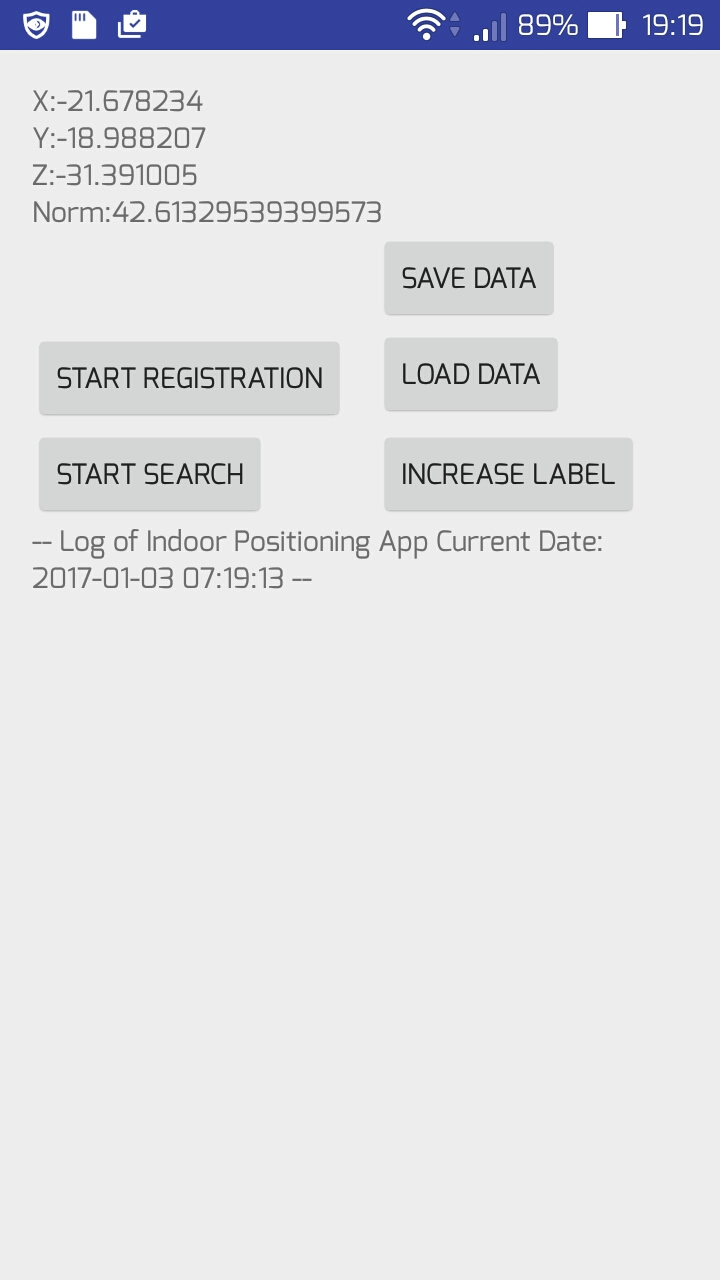
\includegraphics[width=0.3\linewidth]{img/app_screen}
\caption{Interfaccia grafica all'avvio dell'applicazione}
\label{fig:app_screen}
\end{figure}

\begin{figure}[H]
	\centering
	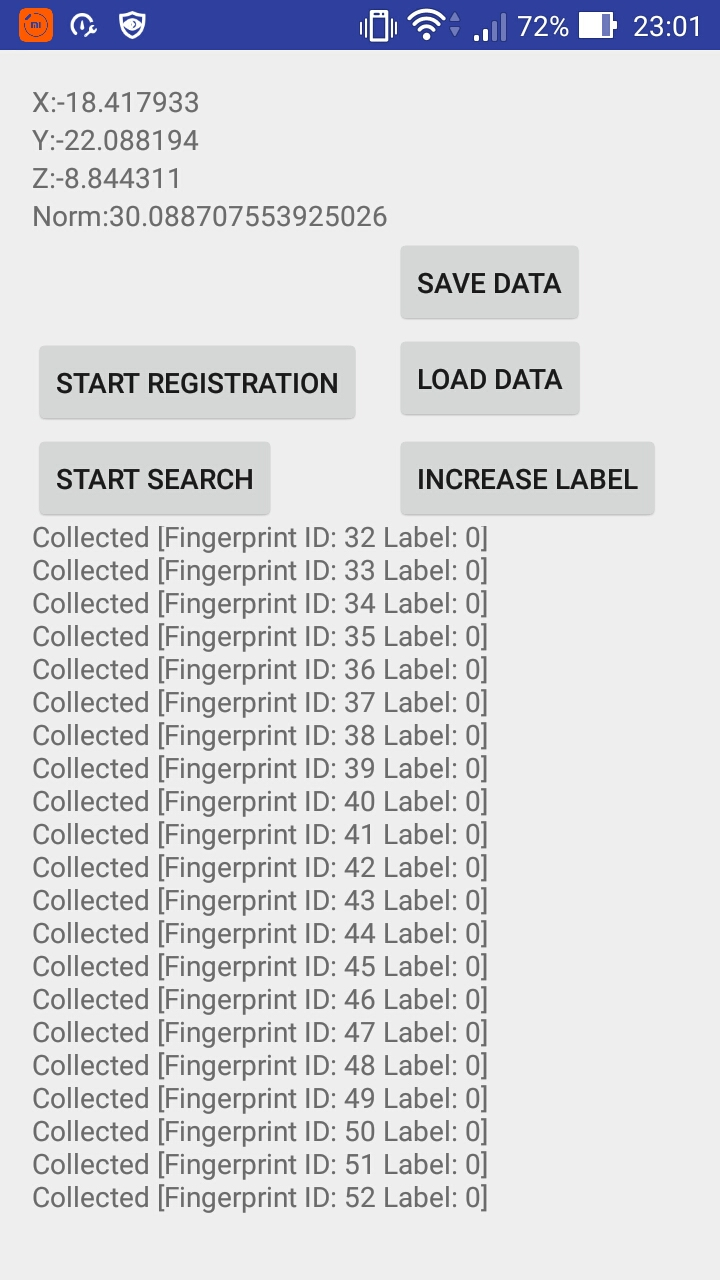
\includegraphics[width=0.7\linewidth]{img/app1}
	\caption{Immagine dell'applicazione durante la raccolta dati}
	\label{fig:app1}
\end{figure}

\begin{figure}[H]
	\centering
	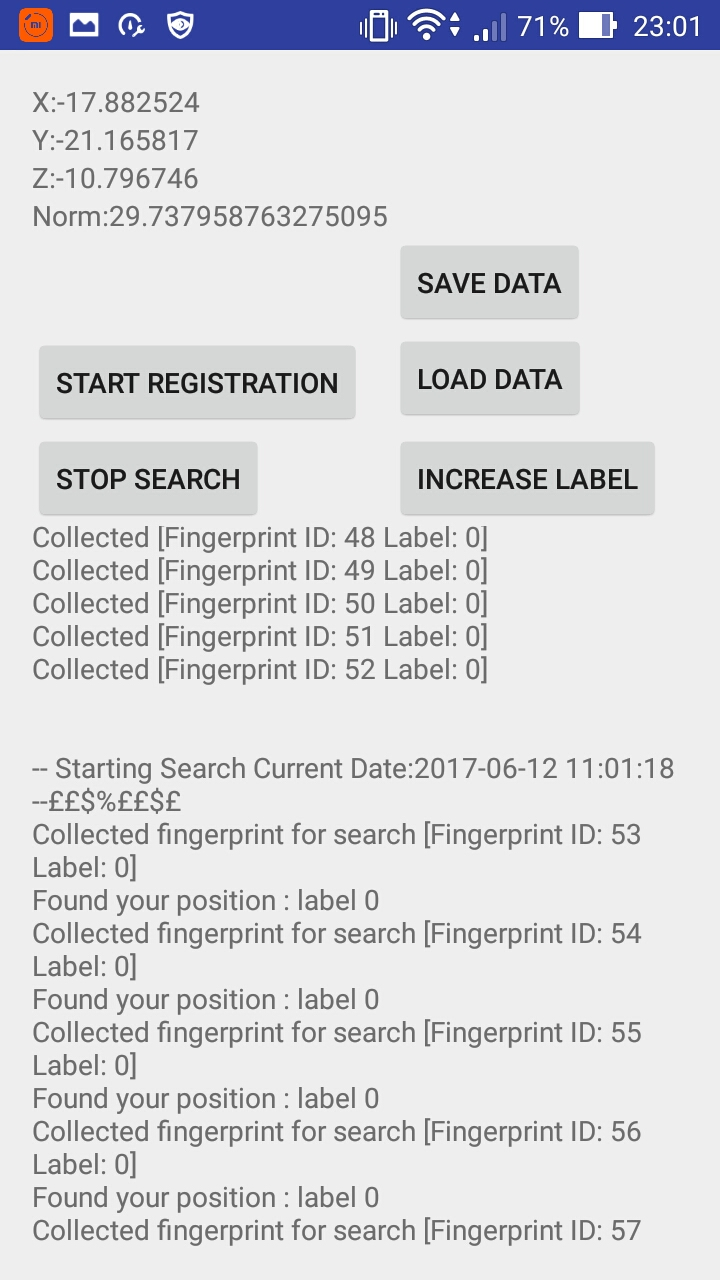
\includegraphics[width=0.7\linewidth]{img/app2}
	\caption{Immagine dell'applicazione durante la ricerca della posizione}
	\label{fig:app2}
\end{figure}


\section{Persistenza dei dati}
L'applicazione consente anche di serializzare tutti i dati registrati fino a quel momento nel formato standard JSON tramite la libreria \textit{gson} che fornisce delle funzioni  per il linguaggio Java per la serializzazione/de-serializzazione di oggetti. Il file viene salvato nella cartella dati dell'applicazione non visibile all'utente.

\section{Struttura del codice e design pattern}
Nello sviluppo del software sono stati applicati vari \textit{design pattern} visti durante i vari corsi e principi di programmazione. Fra questi ultimi abbiamo il \textit{dependency inversion principle}, \textit{open closed principle}. Riguardo i \textit{design pattern}, sono stati usati frequentemente l'\textit{observer}, il \textit{template} e \textit{factory}.

